\documentclass[10pt, a4paper]{article}

% On écrit en français
\usepackage[utf8]{inputenc}
\usepackage[frenchb]{babel}
\usepackage[T1]{fontenc}

% Packages nécessaires
\usepackage{graphicx}
\usepackage{hyperref}

% Numérotation de page custom
\usepackage{fancyhdr}
\usepackage{lastpage}
\pagestyle{fancy}
\fancyhf{}
\rfoot{Page \thepage \hspace{1pt} sur \pageref{LastPage}}

% Police Helvetica <3
\usepackage{helvet}
\renewcommand*{\familydefault}{\sfdefault}

% Enlever les alinéas
\setlength{\parindent}{0pt}

% Marges plus larges pour faire moins LaTeX
\usepackage[left=3cm, right=3cm]{geometry}

% Sous titre de document
\usepackage{titling}
\newcommand{\subtitle}[1]{%
  \posttitle{%
    \par\end{center}
    \begin{center}\large#1\end{center}
    \vskip0.5em}%
}

% En tête complet de document
\newcommand{\Document}[1]{%
    \title{#1}
    \subtitle{Dématérialisation d'un processus de paiement}
    \author{
        COMETS Jean-Marie \\
        DELMARRE Adrian \\
        REYNOLDS Nicolas \\
        TURPIN Pierre
    }
    \date{\today}

    \maketitle \newpage

    \tableofcontents \newpage
}


\begin{document}

\Document{Architecture applicative}

\section{Définition des objets métiers}
La figure \ref{fig:mcd} est le MCD (Modèle Conceptuel de Données) global du
système. Il recense toutes les données utilisées dans le système d'information
de l'étude. \\

\begin{landscape}
  \begin{figure}[ht]
      \centering
      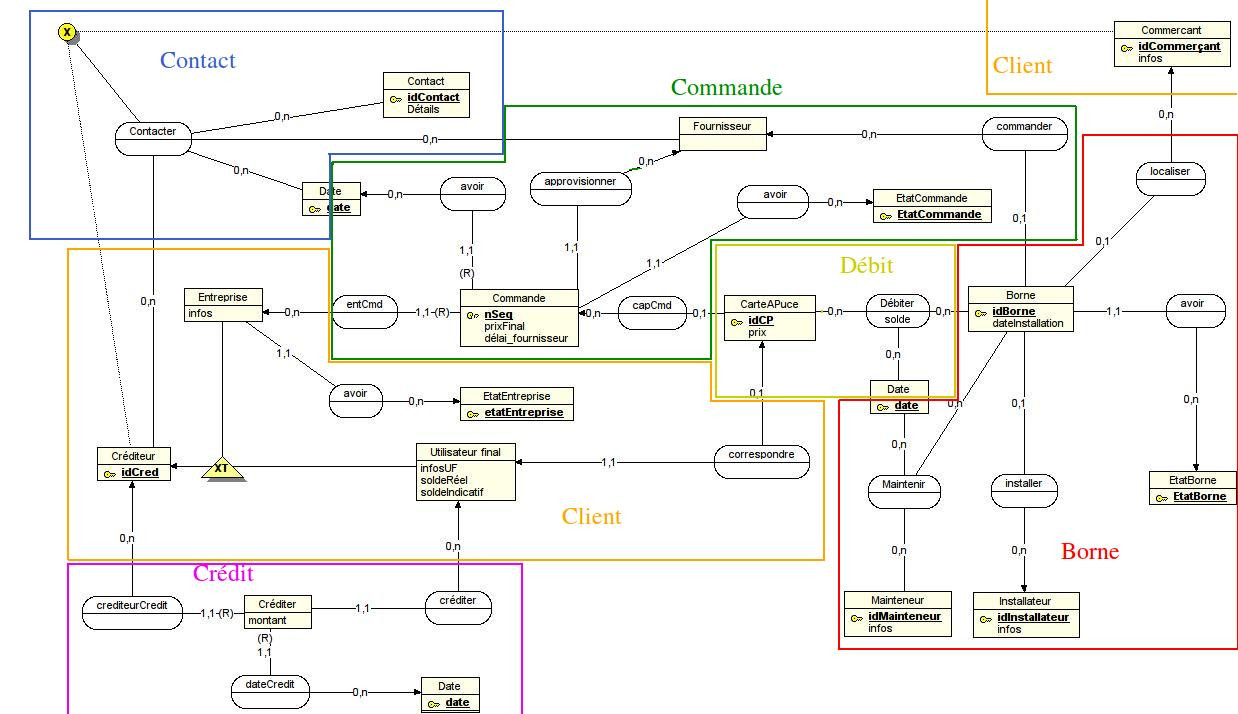
\includegraphics[width=0.7\paperheight]{mcd}
      \caption{MCD global du système}
      \label{fig:mcd}
  \end{figure}
\end{landscape}

Les objets métiers utilisés dans la solution sont les suivants : \\
\begin{description}
  \item[Contact] ...
  \item[Date] ...
  \item[Commande] ...
  \item[Carte à puce] ...
  \item[Borne] ...
  \item[Etat d'une borne] ...
  \item[Fournisseur] ...
  \item[Commercant] ...
  \item[Etat d'une commande] ...
  \item[Entreprise] ...
  \item[Etat d'une entreprise] ...
  \item[Créditeur] ...
  \item[Utilisateur final] ...
  \item[Mainteneur] ...
  \item[Installateur] ...
\end{description}

\section{Extraction des blocs fonctionnels}

\section{Listing des applications utilisateurs}

\section{Génération des services}
\subsection{Services applicatifs}

\subsection{Services métier}

\subsection{Services objet métier}

\section{Description du workflow}

\begin{figure}
  \centering

  \begin{sequencediagram}
      \newthread{acteur}{Acteur~:~Utilisateur final}
      \newinst{ihm}{IHM}
      \newinst{sm}{SM~:~Clients}
      \newinst{som}{SOM~:~Utilisateur final}

      \begin{call}{acteur}{submit(idUF, infosUF)}{ihm}{confirmation}
          \begin{messcall}{ihm}{setInfosUF(id, infos)}{sm}
            \begin{call}{sm}{findById(id)}{som}{found}
            \end{call}
            \begin{sdblock}{IF}{found = VRAI}
              \begin{callself}{sm}{checkInfosUF(infos)}{status,~message}
              \end{callself}
              \begin{sdblock}{IF}{status = OK}
                \begin{call}{sm}{setInfos(id, infos)}{som}{}
                \end{call}
                \begin{mess}{sm}{OK, ACCEPTED}{ihm}
                \end{mess}
              \end{sdblock}
              \begin{sdblock}{ELSE}{status != OK}
                \begin{mess}{sm}{NOT OK, message}{ihm}
                \end{mess}
              \end{sdblock}
            \end{sdblock}
            \begin{sdblock}{ELSE}{found != VRAI}
                \begin{mess}{sm}{NOT OK, NOT FOUND}{ihm}
                \end{mess}
            \end{sdblock}
          \end{messcall}
      \end{call}
  \end{sequencediagram}

  \caption{Modification des informations de l'utilisateurs final}
\end{figure}

\begin{figure}
  \centering

  \begin{sequencediagram}
      \newthread{acteur}{Acteur~:~Utilisateur final}
      \newinst{ihm}{IHM}
      \newinst{sm}{SM~:~Clients}
      \newinst{som}{SOM~:~Utilisateur final}

      \begin{call}{acteur}{submit(loginInfos)}{ihm}{confirmation}
          \begin{messcall}{ihm}{loginUF(loginInfos)}{sm}
            \begin{call}{sm}{findByLoginInfos(loginsInfos)}{som}{id, found}
            \end{call}
            \begin{sdblock}{IF}{found = VRAI}
              \begin{callself}{sm}{connectUF(id)}{}
              \end{callself}
              \begin{mess}{sm}{OK}{ihm}
              \end{mess}
            \end{sdblock}
            \begin{sdblock}{ELSE}{found != VRAI}
                \begin{mess}{sm}{NOT OK}{ihm}
                \end{mess}
            \end{sdblock}
          \end{messcall}
      \end{call}
  \end{sequencediagram}

  \caption{Connexion de l'utilisateur final}
\end{figure}

\begin{figure}
  \centering

  \begin{sequencediagram}
      \newthread{acteur}{Acteur~:~Entreprise}
      \newinst{ihm}{IHM}
      \newinst{sm}{SM~:~Clients}
      \newinst{som}{SOM~:~Utilisateur final}

      \begin{call}{acteur}{submit(idUF)}{ihm}{confirmation}
          \begin{messcall}{ihm}{activateUF(idUF)}{sm}
            \begin{call}{sm}{findById(idUF)}{som}{found}
            \end{call}
            \begin{sdblock}{IF}{found = VRAI}
              \begin{call}{sm}{activate(idUF)}{som}{}
              \end{call}
              \begin{callself}{sm}{notifyUF(idUF)}{}
              \end{callself}
              \begin{mess}{sm}{OK}{ihm}
              \end{mess}
            \end{sdblock}
            \begin{sdblock}{ELSE}{found != VRAI}
                \begin{mess}{sm}{NOT OK}{ihm}
                \end{mess}
            \end{sdblock}
          \end{messcall}
      \end{call}
  \end{sequencediagram}

  \caption{Activation d'un utilisateur final}
\end{figure}

\begin{figure}
  \centering

  \begin{sequencediagram}
      \newthread{acteur}{Acteur~:~Entreprise}
      \newinst{ihm}{IHM}
      \newinst{sm}{SM~:~Clients}
      \newinst{som}{SOM~:~Utilisateur final}
      \newinst{api}{API~:~Banque}

      % \begin{call}{acteur}{submit(idUF)}{ihm}{confirmation}
      %     \begin{messcall}{ihm}{activateUF(idUF)}{sm}
      %       \begin{call}{sm}{findById(idUF)}{som}{found}
      %       \end{call}
      %       \begin{sdblock}{IF}{found = VRAI}
      %         \begin{call}{sm}{activate(idUF)}{som}{}
      %         \end{call}
      %         \begin{callself}{sm}{notifyUF(idUF)}{}
      %         \end{callself}
      %         \begin{mess}{sm}{OK}{ihm}
      %         \end{mess}
      %       \end{sdblock}
      %       \begin{sdblock}{ELSE}{found != VRAI}
      %           \begin{mess}{sm}{NOT OK}{ihm}
      %           \end{mess}
      %       \end{sdblock}
      %     \end{messcall}
      % \end{call}
  \end{sequencediagram}

  \caption{Création d'un utilisateur final}
\end{figure}

\end{document}

% vim: ft=tex et sw=2 sts=2
